% !TeX program = lualatex
\documentclass[10pt,a4paper]{article}

\usepackage[top=20mm,bottom=22mm,left=20mm,right=20mm]{geometry}
\usepackage{fontspec}
\setmainfont{TeX Gyre Termes}
\setsansfont{TeX Gyre Heros}
\setmonofont{Menlo}[Scale=0.82]

\usepackage{amsmath,amssymb}
\usepackage{booktabs}
\usepackage{tabularx}
\usepackage{array}
\usepackage{multirow}
\usepackage{threeparttable}
\usepackage{float}
\usepackage[section]{placeins}
\usepackage{algorithm}
\usepackage{algpseudocode}
\usepackage{siunitx}
\usepackage{xcolor}
\usepackage{enumitem}
\usepackage{tikz}
\usetikzlibrary{arrows.meta,positioning,fit,calc,shapes.geometric,backgrounds}
\usepackage{fontawesome5}
\usepackage{hyperref}
\usepackage[nameinlink,noabbrev]{cleveref}
\makeatletter
\def\theHALG@line{\thealgorithm.\arabic{ALG@line}}
\makeatother
\floatname{algorithm}{Algorithm}
\crefname{algorithm}{Algorithm}{Algorithms}
\algrenewcommand\algorithmicrequire{\textbf{Input:}}
\algrenewcommand\algorithmicensure{\textbf{Output:}}
\algrenewcommand\algorithmicreturn{\textbf{return}}
\usepackage[backend=biber,style=numeric,sorting=none,maxbibnames=99]{biblatex}
\addbibresource{references.bib}
\AtBeginBibliography{\footnotesize}

% Use grayscale throughout for printing and copying.
% Distinctions in figures use shade, line style, and shape rather than hue.
\definecolor{TorPurple}{gray}{0}
\definecolor{TorLight}{gray}{0.94}
\definecolor{EvidenceBlue}{gray}{0.88}
\definecolor{ResultGreen}{gray}{0.82}
\definecolor{LimitRed}{gray}{0.91}
\definecolor{GrayBox}{gray}{0.96}

\hypersetup{
  colorlinks=true,
  linkcolor=black,
  citecolor=black,
  urlcolor=black,
  pdftitle={Memory Forensics of Tor CGO Cryptographic State},
  pdfauthor={Hiro Nakanishi}
}

\setlength{\parindent}{1em}
\setlength{\parskip}{0.25em}
\setlength{\emergencystretch}{2em}
\setlist{nosep,leftmargin=2em}
\renewcommand{\arraystretch}{1.18}
\newcolumntype{Y}{>{\raggedright\arraybackslash}X}
\newcolumntype{L}[1]{>{\raggedright\arraybackslash}p{#1}}
\newcommand{\code}[1]{\nolinkurl{#1}}
\newcommand{\cgo}{\textsc{CGO}}
\newcommand{\torone}{\textsc{TOR1}}
\newcommand{\pcap}{\textsc{PCAP}}
\newcommand{\centralclaim}[1]{%
  \par\noindent\textbf{Central claim: }#1\par
}

\title{\vspace{-8mm}
  \textbf{Memory Forensics of Tor CGO Cryptographic State}\par
  \large Recovering Circuit Ownership and Post-Acquisition Relay Bodies from TLS and CGO State}
\author{Hiro Nakanishi\\Independent Researcher\\\href{mailto:quantumsity@protonmail.com}{quantumsity@protonmail.com}}
\date{}

\begin{document}
\maketitle
\vspace{-5mm}

\begin{abstract}
Counter Galois Onion (CGO) updates cryptographic state for every circuit hop and direction.
Key-like bytes in acquired Tor-client memory do not by themselves establish circuit ownership, entry-oriented hop order, or correspondence with a point in time.
This paper presents a method that starts from C Tor's circuit-ownership list, recovers entry-oriented order from \code{cpath} using matching DWARF information, and follows the circuit to its entry TLS connection. It combines the TLS~1.3 traffic secret and record sequence number with the entry-link circuit identifier and per-hop CGO state to recover a synchronized post-acquisition relay-cell body from a stored PCAP.
Across Tor 0.4.9-series Linux arm64 builds, the analyzer recovered 144/144 controlled circuits and 432/432 hops from 12 independent processes. In 10/10 self-built runs, it verified ownership, TLS AEAD, and unique CGO authentication and recovered a 493-byte body matching evaluation ground truth. A further 6/6 fixed-delay runs reproduced this result across different record numbers and destination hops without pausing the stream or observing cell or TLS-record boundaries. Ground-truth circuit identifiers from the Control Protocol were excluded from candidate selection.
For the stripped Tor 0.4.9.17 package distributed by the Tor Project for Debian 12, the analyzer recovered 36/36 circuits and 108/108 hops in 3/3 structural runs using matching external debug symbols. A replay tool built from the official 0.4.9.17 source recovered a unique CGO-authenticated body in 6/6 traffic runs: 5 DATA cells containing the evaluation marker and 1 SENDME cell.
By contrast, decryption of the immediately preceding cell with the current state failed in 3/3 runs, and sequential acquisition of active endpoints produced 0/36 state matches after gaps of 2.30--3.17 seconds.
The method therefore establishes correspondences among circuits, paths, cryptographic schemes, and synchronized post-acquisition traffic content. It does not provide comprehensive decryption of past traffic or remote deanonymization of Tor.

\noindent\textbf{Keywords:} Tor, Counter Galois Onion, memory forensics, core dump, TLS, offline decryption
\end{abstract}

\section{Introduction}

Tor makes it difficult to link a communication source to its destination by using circuits through multiple relays and layered cryptographic processing~\cite{dingledine2004tor}.
This property protects ordinary communications. When investigating a compromised endpoint, however, the questions are where the state of each circuit resides in acquired memory and what can be recovered from that state.

CGO introduces authenticated onion encryption into Tor and updates keys, nonces, and an accumulated state $T'$ as cells are processed~\cite{torproposal359,degabriele2025cgo}.
These updates make a simple key search insufficient. Finding a CGO structure in memory does not reveal whether it belongs to an open circuit, which hop it represents, or to cells at which point in time it applies.

This study addresses the following question.

\begin{quote}
\textbf{Research question:} Under what conditions, and to what extent, can CGO/\torone{} circuit state and traffic content be recovered offline from a core dump and related evidence acquired during controlled, ongoing communication by an unmodified C Tor process?
\end{quote}

\centralclaim{When the TLS write-record sequence number retained in a core dump matches the first post-acquisition record that can be authenticated in a stored PCAP, circuit ownership, entry-oriented hop order, entry TLS, and per-hop CGO state can be associated, and the body of the relay cell in that record that passes CGO authentication can be recovered. This is a forensic method available after endpoint-memory acquisition, not an attack that breaks CGO itself.}

Section~\ref{sec:contributions} summarizes the contributions, Section~\ref{sec:background} describes CGO and the investigation target, and Section~\ref{sec:related} distinguishes this work from prior research. Section~\ref{sec:method} presents the evidence-based method, Section~\ref{sec:implementation} its evaluation implementation, Section~\ref{sec:experiment} the experimental design, and Section~\ref{sec:results} the results. Section~\ref{sec:security} examines the attack-capability boundary created by extracted state, and Sections~\ref{sec:discussion} and~\ref{sec:limitations} discuss practical implications and limitations.

The analyzer, experimental scripts, and evaluation results with sensitive information removed are available in a public repository\footnote{Implementation and supplementary material: \url{https://github.com/quantumshiro/tor-cgo-analysis}}.

\section{Contributions}\label{sec:contributions}

The contributions of this study are summarized in four points.

\begin{enumerate}[label=\textbf{C\arabic*.},leftmargin=3em]
  \item \textbf{Static memory analysis rooted in circuit ownership.}
  Rather than scanning for key or structure patterns, the method enumerates client-originated circuits (origin circuits) from Tor's own ownership list. It treats \code{origin_circuit_t.cpath} as the entry and checks magic values, list indices, bidirectional links, and cycle closure, thereby verifying both circuit ownership and entry-oriented hop order. Across 12 independent processes spanning multiple versions and optimization conditions, it recovered 144/144 controlled circuits and 432/432 hops. It also recovered 36/36 circuits and 108/108 hops from 3 independent processes of the distributed package build.

  \item \textbf{Correspondence among circuits, TLS, and CGO state.}
  Following pointer relationships among Tor structures, the method associates circuit identifiers, stream destinations, entry channels, per-hop CGO/\torone{} schemes, and per-direction CGO state. Unlike a method that merely finds key-like values in memory, it can therefore explain to which circuit, hop, and direction each state belongs.

  \item \textbf{Recovery of synchronized post-acquisition traffic by processing TLS records and the CGO layer in sequence.}
  The method identifies the entry OpenSSL object from an owned circuit and obtains the TLS~1.3 traffic secret and write-record sequence number. Traffic recovery is limited to all-CGO circuits whose ownership, path structure, and cryptographic contexts can be verified. It then performs authenticated TLS decryption of the PCAP, enumerates every Tor-cell candidate, and processes the CGO layer in that order. For self-built Tor, it recovered a unique CGO-authenticated relay-cell body in 10/10 independent runs that paused communication and in 6/6 fixed-delay runs that neither stopped the stream nor observed cell or TLS boundaries. For the official package build, CGO authentication also succeeded in 6/6 runs, while relay DATA cells containing the evaluation marker were obtained in 5/6. Ground truth from the Control Protocol or dynamic instrumentation was excluded from decryption inputs and used only for evaluation after candidate selection.

  \item \textbf{Quantification of success conditions and false-attribution boundaries.}
  Negative controls covered uninitialized enum values during construction, missing pages, a mismatched executable, wrong keys, acquisition-time mismatch, the immediately preceding cell, and a known backward-direction resynchronization attack. The results show that current state can be used for the next cell after core-dump acquisition, but does not imply comprehensive decryption of past traffic, a remote attack, or general deanonymization.
\end{enumerate}

These contributions do not constitute new cryptanalysis of CGO. The CGO-specific contribution is to attribute per-hop evolving authenticated state sequences to circuits and points in time, then apply them to synchronized post-acquisition traffic in the correct order. The more general contribution is a method that starts from ownership structures, progressively combines type information, transport-layer authenticated state, and higher-layer cryptographic state, and records whether each check succeeded, failed, or was not evaluated.

\section{Background}\label{sec:background}

\subsection{Tor Circuits and Relay Cells}

Tor clients normally construct circuits by selecting entry, middle, and exit relays in that order.
For forward cells sent by the client, cryptographic layers are applied from the exit toward the entry. Received backward cells are processed in the opposite direction.
Because cells are carried over the TLS connection to the entry, packets observed on the network are protected by both the TLS and onion layers.

A C Tor origin circuit holds the circuit identifier, entry channel, streams, and path~\cite{ctorsource04916}.
The path is a circular doubly linked list of \code{crypt_path_t} objects.
Crucially, the lowest address in the list is not the entry; \code{origin_circuit_t.cpath} points to the entry hop.
No inference from address order is therefore needed, because orientation follows from the semantics of the ownership structure.

\subsection{CGO State and the Direction of Time}

Proposal~359 defines CGO processing for the 509 bytes of a relay cell~\cite{torproposal359}.
Each hop and direction retains a pseudorandom-function key $K$, a nonce $N$, and an accumulated value $T'$ used for authentication, among other values.
CGO updates its state whenever it processes a cell. Conceptually, state $S_i$ and cell $C_i$ produce output and the next state.

CGO was released in C Tor 0.4.9.5 as a stable feature that clients and relays can negotiate, although Proposal~359 itself remained Open at the time of writing~\cite{torstable0495,torproposal359}. Versions 0.4.9.3-alpha through 0.4.9.11 also contained an implementation defect that failed to enable congestion control, and consequently failed to negotiate CGO, on hops other than the final hop. Version 0.4.9.12 corrected this behavior so that congestion control and CGO are negotiated on every supporting hop~\cite{torrelease04912}. Thus, mixed schemes depend not only on relay capabilities but also on the client version and circuit-construction conditions. Because an enum value alone cannot identify an established cryptographic scheme, the method also verifies whether each hop's cryptographic context was initialized at acquisition time.

\begin{equation}
  (C'_i, S_{i+1}) = \operatorname{CGO}(C_i,S_i).
\end{equation}

A snapshot retains $S_t$ at acquisition time. Starting from $S_t$, future cells synchronized to that state can be processed sequentially. By contrast, the immediately preceding cell $C_{t-1}$ cannot be decrypted unless the pre-update state $S_{t-1}$ remains available. This direction of time differs from the recovery of an ordinary disk-encryption key.

\begin{figure}[t]
\centering
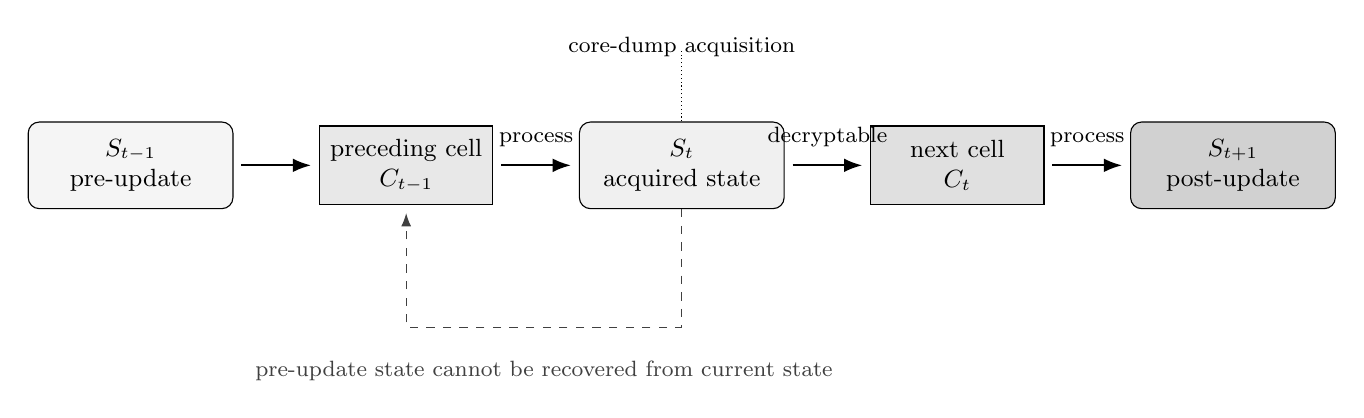
\begin{tikzpicture}[
  x=1mm,y=1mm,>=Latex,
  state/.style={draw,rounded corners,minimum width=26mm,minimum height=11mm,align=center,font=\small},
  cell/.style={draw,minimum width=22mm,minimum height=10mm,align=center,font=\small},
  note/.style={font=\footnotesize,align=center}
]
\node[state,fill=GrayBox] (s0) at (0,0) {$S_{t-1}$\\pre-update};
\node[cell,fill=LimitRed] (past) at (35,0) {preceding cell\\$C_{t-1}$};
\node[state,fill=TorLight] (st) at (70,0) {$S_t$\\acquired state};
\node[cell,fill=EvidenceBlue] (next) at (105,0) {next cell\\$C_t$};
\node[state,fill=ResultGreen] (s1) at (140,0) {$S_{t+1}$\\post-update};
\draw[->,thick,shorten <=1mm,shorten >=1mm] (s0) -- (past);
\draw[->,thick,shorten <=1mm,shorten >=1mm] (past) -- node[above=1mm,note]{process} (st);
\draw[->,thick,shorten <=1mm,shorten >=1mm] (st) -- node[above=1mm,note]{decryptable} (next);
\draw[->,thick,shorten <=1mm,shorten >=1mm] (next) -- node[above=1mm,note]{process} (s1);
\coordinate (rollback) at ($(st.south)+(0,-15mm)$);
\draw[->,dashed,black!75,shorten >=1mm] (st.south) -- (rollback) -| (past.south);
\coordinate (rollbacklabel) at ($(past.south |- rollback)!0.5!(rollback)$);
\node[note,text=black!75,below=3mm of rollbacklabel] {pre-update state cannot be recovered from current state};
\node[note,above=7mm of st] {core-dump acquisition};
\draw[densely dotted] (st.north) -- ++(0,9mm);
\end{tikzpicture}
\caption{Temporal boundary of CGO state. Current state can process the synchronized next cell but generally cannot process the immediately preceding cell once pre-update state is lost.}
\label{fig:time}
\end{figure}


The Tor Control Protocol can query a running Tor process for circuit identifiers, paths, stream states, and related information~\cite{torcontrol}.
It does not expose per-hop CGO/\torone{} objects, TLS traffic secrets internal to OpenSSL, or per-direction CGO state.
Nor can it connect to a core dump after process termination.
Control Protocol records are used only as evaluation ground truth and are excluded from analysis inputs.

\section{Related Work}\label{sec:related}

\subsection{Onion Encryption and CGO}

Early Tor made low-latency onion routing practical, but the modification resistance of its relay cryptography presented formal challenges~\cite{dingledine2004tor}.
Degabriele and Stam formalized onion encryption and analyzed Tor relay cryptography against security definitions~\cite{degabriele2018untagging}.
Degabriele et al. subsequently proposed CGO to combine authentication with high-speed processing and reported its construction and performance~\cite{degabriele2025cgo}.
Security models incorporating leaky pipes, associated data, and partial forward secrecy have also been studied~\cite{degabriele2025secure}.

These studies address cryptographic security and state transitions, but not how to attribute state in acquired real-process memory to a circuit that owned it at acquisition time.
Proposal~359 likewise defines state that an implementation must retain, but does not address forensic acquisition, missing pages, ABI differences, or evidentiary linkage with TLS~\cite{torproposal359}.

\subsection{Memory Forensics of Tor, Cryptographic Keys, and TLS}

Alfosail and Norris proposed an investigative procedure for traces remaining in Tor client memory~\cite{alfosail2021tor}.
Muir et al. audited the Tor Browser Bundle and evaluated usage traces left on Windows hosts~\cite{muir2019forensic}.
Arshad et al. compared traces in the registry, storage, memory, and Zram on Windows~10 and Android~10~\cite{arshad2021forensic}.
These studies are useful for establishing Tor use and collecting endpoint artifacts, but do not investigate C Tor's internal circuit ownership, entry-oriented cryptographic paths, per-hop CGO state, or layer-by-layer recovery from TLS through CGO.

The Tor Project has also analyzed the privacy implications of statistics retained in memory~\cite{tor2017memory}.
That work concerns minimizing in-memory information by design, whereas this study interprets cryptographic state of client circuits after acquisition.


Research on finding cryptographic keys in RAM has shown that the structure of a key schedule can identify keys for AES and other ciphers~\cite{maartmannmoe2009persistence}.
Cold-boot research demonstrated that keys can be reconstructed from degraded RAM~\cite{halderman2008coldboot}.
These results establish that cryptographic state can constitute memory evidence.
Finding a key alone, however, does not reveal which Tor circuit, hop, and direction owns it.
This study therefore begins with Tor ownership relationships rather than with a key search and follows them to cryptographic state.


X-Ray-TLS extracts TLS~1.2, TLS~1.3, and QUIC session secrets from process memory and transparently decrypts traffic~\cite{moriconi2024xraytls}. Baier et al. systematized methods for identifying and extracting TLS key material from memory and surveyed implementation differences, TLS~1.3, and post-acquisition analysis challenges~\cite{baier2024tlsmemory}. A further method locates key-derivation functions from standard-specific strings and hooks major TLS implementations~\cite{baier2025allyourtlskeys}. This adjacent work is important because it precludes claiming TLS-secret extraction itself as novel here.

Even after obtaining TLS plaintext for the entry link, relay cells within it remain protected by per-hop CGO layers. A TLS secret alone also does not identify which Tor-owned circuit, entry-oriented hop, or acquisition-time CGO state should be applied. The distinction of this study is not TLS-secret extraction; it is the association of the TLS object, link circuit identifier, per-hop CGO state, and acquisition time from pointer relationships among Tor structures. Table~\ref{tab:related-matrix} summarizes the investigative differences.

\begin{table}[!tbp]
\centering
\caption{Investigative scope addressed by related methods}
\label{tab:related-matrix}
\small
\begin{tabularx}{\linewidth}{Yccccc}
\toprule
Method & Tor-owned circuits & Entry order & TLS decryption & CGO decryption & TLS-sequence/CGO-state association \\
\midrule
Tor endpoint-trace studies~\cite{alfosail2021tor,muir2019forensic} & -- & -- & -- & -- & -- \\
Generic key search~\cite{maartmannmoe2009persistence} & -- & -- & -- & -- & -- \\
X-Ray-TLS~\cite{moriconi2024xraytls} & -- & -- & $\checkmark$ & -- & -- \\
TLS-key extraction and surveys~\cite{baier2024tlsmemory,baier2025allyourtlskeys} & -- & -- & $\checkmark$ & -- & -- \\
This method & $\checkmark$ & $\checkmark$ & $\checkmark$ & $\checkmark$ & $\checkmark$ \\
\bottomrule
\end{tabularx}
\end{table}

In practice, a lighter method may satisfy an investigation's objective. A DFRWS EU 2026 exercise addresses capturing localhost traffic before it enters Tor and analyzing information corresponding to the inside of the encrypted Tor tunnel~\cite{dfrws2026localtor}. This is a strong option when loopback capture was arranged in advance, and it is simpler than the present method if application content alone is the objective. Determining which Tor circuit, hop, and cryptographic scheme carried that traffic, or what can be established from a subsequently acquired core, is a separate problem. Table~\ref{tab:practical-alternatives} distinguishes the method from acquisition alternatives that compete in operational use.

\begin{table}[!tbp]
\centering
\caption{Comparison with practical alternatives}
\label{tab:practical-alternatives}
\small
\begin{tabularx}{\linewidth}{L{28mm}Y Y L{25mm}}
\toprule
Method & Principal information obtained & Principal information not obtained & Suitable situation \\
\midrule
Ordinary logs / Control Protocol & Live circuit IDs, paths, and stream state & Per-hop cryptographic contexts, TLS secrets, post-termination reanalysis & A live process can be queried immediately \\
localhost/SOCKS-side PCAP~\cite{dfrws2026localtor} & Application traffic before entering Tor & Attribution to an onion circuit, hop schemes, cells on entry link & Prior capture exists and content is the objective \\
Generic TLS-key extraction~\cite{moriconi2024xraytls,baier2024tlsmemory} & Tor cells within entry TLS & CGO-layer relay-cell body, owned circuit, entry order & Only TLS internals need inspection \\
This method with core dump alone & Owned circuits, entry order, and CGO/\torone{} state at acquisition & Traffic content & Post-incident analysis with only a core dump \\
This method with core dump and PCAP & Above, plus TLS cells and CGO-authenticated relay-cell bodies whose acquisition-time correspondence is verified & Arbitrary past traffic; automatic removal of upper-layer encryption & Core dump and entry PCAP correspond to the same acquisition point \\
\bottomrule
\end{tabularx}
\end{table}

\subsection{Previously Unresolved Investigative Gap}

The unresolved issue in prior work is not finding cryptographic state, but attributing that state and placing it in time.
The Control Protocol can describe circuits in a live process but does not provide internal cryptographic state or post-acquisition analysis.
Tor forensic research addresses endpoint traces but not the semantics of CGO state.
Cryptographic-key and TLS forensics obtain keys or TLS plaintext but do not recover Tor circuit ownership and the CGO layer.

The novelty of this work is to establish these three elements as a verifiable correspondence. It identifies a target circuit from Tor's internal ownership relationships, orders its hops from the entry, and applies TLS and CGO state held by the same circuit to a synchronized post-acquisition record in a stored PCAP. This combination distinguishes structurally plausible remnants from state owned at acquisition time and reaches the relay body.

\section{Proposed Method}\label{sec:method}

\subsection{Overview and Analysis Problem}

The method does not search the entire memory image for cryptographic keys. Instead, it follows ownership relationships maintained by Tor in the forward direction and reaches cryptographic state last. The analysis order is to \textbf{identify owned circuits}, \textbf{identify the entry and hop order}, \textbf{establish the cryptographic scheme and initialization state}, \textbf{extract TLS and CGO secrets}, and \textbf{match them to synchronized post-acquisition traffic}.

This order matters. The heap may retain structures from closed circuits, zero-initialized regions for circuits under construction, freed keys, and OpenSSL contexts belonging to other circuits. If only cryptographic values are found first, their circuit ownership cannot later be established. The method begins at \code{global_origin_circuit_list}, maintained by Tor itself. A structure or key that cannot be reached from that list cannot be attributed to a circuit owned at acquisition time, even if its value appears cryptographically plausible.

The attainable result depends on whether a PCAP is available. From only a core dump, matching executable, and DWARF, the method recovers circuits owned at acquisition time, their lifecycle, entry-oriented paths, stream destinations, per-hop CGO/\torone{} schemes, and per-direction CGO state. The target process may already have terminated.

If a PCAP records the entry link across the core-dump acquisition point, the method also authenticates the record corresponding to the TLS write-record sequence number in the core and applies CGO state to Tor cells within it. This traffic analysis is suitable when Tor can resume after core-dump acquisition. If only a crash dump exists and there is no subsequent traffic, analysis stops at circuit state. Current CGO state cannot be rolled back to cells before acquisition unless a separate copy of the pre-update state remains.


\paragraph{Threat model and trust boundary.}
The investigator is assumed to have lawful authority to acquire the target endpoint and to trust the acquisition tool, analyzer, and hashing environment. The core dump and PCAP are assumed not to have been modified after acquisition; candidate ELF/DWARF files must pass compatibility checks against core mappings; and the OpenSSL-internal profile must have been validated for the target build. Even when the target process has been compromised, remnant structures, uninitialized regions, and partial loss are included in the checks. Out of scope is anti-forensic fabrication by an attacker who, before acquisition, can arbitrarily rewrite memory and deliberately make Tor's ownership list, circuit structures, cryptographic state, and PCAP mutually consistent.

Membership in the ownership list and structural validation show that Tor's ownership relationships and state are internally consistent within the acquired evidence. They do not replace legal chain-of-custody procedures. Verification of TLS and CGO authentication tags shows that the target bytes authenticate under the extracted secrets; it does not show that a particular person intended the communication or attribute an origin outside the endpoint. Result records include acquisition time, input hashes, success, failure, or non-evaluation for every check, and the reason for each status.

The required inputs are a core dump $M_t$ of the Tor process acquired at time $t$ and type information $B$ corresponding to the executable that produced $M_t$. A core dump is a post-acquisition snapshot containing the process's virtual memory and registers. The candidate ELF Build ID is recorded. When the core does not retain an exact Build ID, $B$ is accepted only as a compatible candidate if at least 75\% of corresponding bytes match between the main executable region identified by the core's \code{NT_FILE} mapping and the candidate ELF, as specified in Section~\ref{sec:implementation}. This comparison is not treated as proof of executable identity. Only when post-acquisition traffic is to be recovered is a packet capture $P$ of the client--entry link spanning time $t$ added.

The unit of analysis is an origin circuit. For each circuit $c$, the method produces the following result record $R_c$.

\begin{equation}
R_c=(I_c,L_c,H_c,A_c,Q_c,U_c,Z_c,V_c).
\label{eq:result-record}
\end{equation}

$I_c$ comprises Tor's internal circuit identifier and the circuit ID on the entry link; $L_c$ is the lifecycle, such as building, established, or marked for close; and $H_c=(h_0,\ldots,h_{n-1})$ is the hop sequence ordered from the entry. $A_c$ contains streams owned by the circuit and their destinations; $Q_c$ records the established cryptographic scheme and whether accumulated CGO state has changed for every hop and direction; $U_c$ records the correspondence of TLS records and CGO state to the core-dump acquisition point; and $Z_c$ is a recovered Tor cell or relay-cell body. $V_c$ records complete ownership-list enumeration, circuit structure, cryptographic context, TLS AEAD, and CGO authentication as success, failure, or not evaluated, together with reasons. A field whose input is missing or whose validation fails is marked not evaluated and given a reason.

The one-direction CGO state defined by Proposal~359 is represented as the following logical value rather than by implementation addresses~\cite{torproposal359}.

\begin{equation}
S_{c,d,h}(t)=(K_J,H_J,K_S,H_S,N,T').
\label{eq:cgo-state}
\end{equation}

$c$ is the circuit, $d$ is the forward or backward direction, $h$ is the hop, and $t$ is the acquisition time. $K_J$ and $K_S$ are two AES-128 keys, $H_J$ and $H_S$ are two POLYVAL keys, $N$ is a nonce, and $T'$ is accumulated state updated by cell processing. Each component is 16 bytes, for a total of 96 bytes per direction. The analysis must attribute this logical value to a circuit, direction, and hop. Circuit attribution and entry ordering do not depend on memory-address order or fixed offsets. Extraction of secrets from OpenSSL internals, however, depends on the version-specific profiles described later.

\subsection{Procedure from Ownership to Traffic Recovery}

The method is divided into circuit-state recovery from a core dump alone (Algorithm~\ref{alg:core-recovery}) and traffic recovery with an additional stored PCAP (Algorithm~\ref{alg:traffic-recovery}). Every preceding validation must succeed before a processing stage is considered established. Success at a later stage does not compensate for an unestablished earlier stage.

The ownership list $O_t$ is read in full, and the element $c$ at position $j$ becomes an analysis target. The condition for validating structure-membership information is
\begin{equation}
\operatorname{Structured}(c,j)=
[\operatorname{idx}(c)=j]\land[\operatorname{magic}(c)=M_{\mathrm{origin}}].
\label{eq:structured}
\end{equation}

In the algorithms, \textsc{VerifyExecutable} records the candidate ELF Build ID and compares bytes corresponding between the ELF and the main executable region identified by the core dump's \code{NT_FILE}. \textsc{SafeRead} returns a typed value only when the target range is readable; otherwise it returns a failure reason. After these checks, \textsc{RecoverOwnedMetadata} recovers circuit identifiers, lifecycle, and owned streams. \textsc{RecoverCryptoState} recovers each hop's scheme identifier, forward and backward cryptographic contexts, and the CGO state in Equation~\eqref{eq:cgo-state}. Proposal~359 initializes $T'$ to zero and updates it during subsequent cell processing, so $T'\neq0$ is separately recorded as evidence that $T'$ in that direction has changed from its initial value~\cite{torproposal359,ctorsource04916}.

\textsc{AuthenticateExactSequence} verifies TLS Authenticated Encryption with Associated Data (AEAD) using only the write-record sequence number stored in the core dump. \textsc{EnumerateRelayCells} returns every cell of the target circuit contained in the authenticated record; it does not narrow the set to one by using a ground-truth circuit ID from the Control Protocol. \textsc{ApplyCGOFromSnapshot} applies each candidate, in entry order, to a copy of the same acquisition-time state and returns the hop that recognized the CGO authentication tag and the 493-byte relay body excluding the tag~\cite{torproposal359}.
Complete enumeration of the ownership list and structural validation of each circuit are recorded separately. Thus, even when a circuit structure is corrupt, the observation that its pointer appeared in the ownership list at acquisition time is retained.
The entry-oriented hop sequence is recovered by setting $h_0=c.\mathrm{cpath}$ and $h_{i+1}=\operatorname{next}(h_i)$. Mutual consistency of forward and backward links is checked at each hop, and the cycle is accepted only if the sequence returns to $h_0$.

When processing a stored PCAP, let the TLS~1.3 traffic secret be $S$ and the record sequence number be $i$. The key $k$, initialization vector $v$, and nonce $n_i$ are derived according to RFC~8446~\cite{rfc8446}. The hash $\mathcal H$ and key length $\ell$ are determined by the cipher suite; for \code{TLS_AES_256_GCM_SHA384} used in this evaluation, $\mathcal H=\mathrm{SHA384}$ and $\ell=32$.
\begin{align}
  k &= \operatorname{HKDF\mbox{-}Expand\mbox{-}Label}_{\mathcal H}(S,\mathrm{key},\ell),\label{eq:tls-key}\\
  v &= \operatorname{HKDF\mbox{-}Expand\mbox{-}Label}_{\mathcal H}(S,\mathrm{iv},12),\\
  n_i &= v \oplus \operatorname{I2OSP}_{12}(i).
\end{align}

\begin{algorithm}[H]
\caption{Circuit-state recovery rooted in ownership}
\label{alg:core-recovery}
\small
\begin{algorithmic}[1]
\Require Core dump $M_t$; candidate executable and type information $B$
\Ensure Set of per-circuit result records $\mathcal{R}=\{R_c\}$
\State $\mathcal{R}\gets\emptyset$
\If{$\Call{VerifyExecutable}{M_t,B}$ fails}
  \State \Return $\{\operatorname{error}(\text{executable mismatch})\}$
\EndIf
\State $\Lambda\gets\Call{ResolveTypes}{B}$
\State $O_t\gets\Call{ReadOwnerList}{M_t,\Lambda}$
\If{the region, count, capacity, or any element of $O_t$ cannot be verified}
  \State \Return $\{\operatorname{incomplete}(\text{ownership list unavailable})\}$
\EndIf
\For{$j\gets0$ \textbf{to} $|O_t|-1$}
  \State $(I_c,L_c,H_c,A_c,Q_c,U_c,Z_c,V_c)\gets(\bot,\bot,\bot,\bot,\bot,\bot,\bot,\emptyset)$
  \State $c\gets O_t[j]$; record membership in ownership list
  \If{$\Call{SafeRead}{M_t,c,\Lambda}$ fails}
    \State record reason for circuit-structure failure in $V_c$
    \State $R_c\gets(I_c,L_c,H_c,A_c,Q_c,U_c,Z_c,V_c)$; $\mathcal{R}\gets\mathcal{R}\cup\{R_c\}$; \textbf{continue}
  \EndIf
  \If{$\operatorname{Structured}(c,j)$}
    \State $(I_c,L_c,A_c)\gets\Call{RecoverOwnedMetadata}{c}$
    \State $H_c\gets\Call{WalkFromEntry}{c.\mathrm{cpath}}$
  \EndIf
  \If{$\operatorname{Structured}(c,j)$ and $H_c$ passes bidirectional-link and cycle checks}
    \State record successful validation of circuit structure and entry-oriented path
    \State $Q_c\gets\Call{RecoverCryptoState}{c,H_c}$
    \If{circuit is active and established, and scheme-specific contexts are consistent at all hops}
      \State record successful validation of cryptographic-context initialization
    \EndIf
  \EndIf
  \State mark unexecuted later checks not evaluated in $V_c$ and record reasons
  \State $R_c\gets(I_c,L_c,H_c,A_c,Q_c,U_c,Z_c,V_c)$
  \State $\mathcal{R}\gets\mathcal{R}\cup\{R_c\}$
\EndFor
\State \Return $\mathcal{R}$
\end{algorithmic}
\end{algorithm}

For the forward direction, define all per-hop states from entry through exit as
\begin{equation}
\mathcal{S}_{c,\mathrm{forward}}(t)=
\bigl(S_{c,\mathrm{forward},0}(t),\ldots,
S_{c,\mathrm{forward},n-1}(t)\bigr)
\label{eq:cgo-state-sequence}
\end{equation}
For each candidate cell, this state sequence is copied and applied to each layer in the same entry order as Tor's forward processing. If CGO authentication succeeds at a hop, that hop is returned as the destination. Thus, \textsc{ApplyCGOFromSnapshot} below receives the full state sequence of Equation~\eqref{eq:cgo-state-sequence}, not only the state of the entry hop.

\begin{algorithm}[H]
\caption{Post-acquisition traffic recovery by sequential TLS and CGO processing}
\label{alg:traffic-recovery}
\small
\begin{algorithmic}[1]
\Require $\mathcal{R}$; core dump $M_t$; stored PCAP $P$ containing the entry link
\Ensure $\mathcal{R}$ augmented with TLS and CGO validation results
\ForAll{$R_c\in\mathcal{R}$ with validated ownership, path, and cryptographic contexts, and CGO at every hop}
  \State $T_c\gets\Call{RecoverEntryTLS}{M_t,c}$
  \If{TLS version, role, cipher suite, secret length, and circuit attribution of $T_c$ validate}
    \State $\mathcal{D}_c\gets\Call{AuthenticateExactSequence}{P,T_c,T_c.\mathrm{write\_seq}}$
    \State $\mathcal{C}_c\gets\Call{EnumerateRelayCells}{\mathcal{D}_c,I_c.\mathrm{link\_circid}}$
    \If{$\mathcal{C}_c\neq\emptyset$}
      \State record successful TLS AEAD and cell extraction; $U_c\gets(T_c.\mathrm{write\_seq},\mathcal{D}_c)$
      \State $\mathcal{A}_c\gets\emptyset$
      \ForAll{$q\in\mathcal{C}_c$ in PCAP order}
        \State $\widehat{\mathcal{S}}\gets\Call{Copy}{\mathcal{S}_{c,\mathrm{forward}}(t)}$
        \State $(h,z)\gets\Call{ApplyCGOFromSnapshot}{q,H_c,\widehat{\mathcal{S}}}$
        \If{CGO authentication tag is recognized at $h$}
          \State $\mathcal{A}_c\gets\mathcal{A}_c\cup\{(q,h,z)\}$
        \EndIf
      \EndFor
      \If{$|\mathcal{A}_c|=1$}
        \State record successful CGO authentication; $Z_c\gets\operatorname{only}(\mathcal{A}_c)$
      \EndIf
    \EndIf
  \EndIf
\EndFor
\State \Return $\mathcal{R}$
\end{algorithmic}
\end{algorithm}

If CGO-tag validation fails for every candidate, or succeeds for more than one candidate, the destination hop and relay-cell body cannot be uniquely identified. Structural validation, TLS authentication, and CGO authentication are validation conditions based on different state and keys. Their statistical independence is not assumed. Plaintext recovery is established only when all three validations succeed; success of any one alone is insufficient.

\subsection{Validation Items and Decision Criteria}

The target is a C Tor client running on an endpoint that the investigator is authorized to examine.
Inputs are (1) an ELF core dump and (2) the executable and DWARF whose Build ID is recorded and whose compatibility with executable mappings in the core has been verified. Validation of TLS and CGO authentication additionally requires (3) an entry-link PCAP spanning the acquisition point.
Analysis is performed after acquisition; no dynamic debugger or special identifier is embedded in the target process.

Successful recovery is defined not by merely producing a candidate, but by passing the following checks.

\begin{itemize}
  \item The circuit appears in Tor's own origin-circuit ownership list.
  \item List index, magic value, pointer ranges, \code{next}/\code{prev}, and cycle closure are consistent.
  \item Lifecycle and initialization of cryptographic state are consistent.
  \item For PCAP decryption, TLS AEAD authentication, the Tor circuit ID, and CGO tag recognition succeed in sequence. In evaluation experiments, the recovered body is compared with separately acquired ground-truth plaintext.
\end{itemize}

Control Protocol records, dynamically hooked cells, and synthetic identities obtained through additional instrumentation are evaluation-only ground truth and are excluded from analysis inputs.

For every item in Table~\ref{tab:evidence-levels}, each check records success, failure, or not evaluated. A later stage executes only if every prerequisite check succeeded. Success of CGO authentication alone does not establish circuit recovery if the ownership list and \code{cpath} cannot be validated.

\begin{table}[!tbp]
\centering
\caption{Validation items recorded in analysis results}
\label{tab:evidence-levels}
\small
\begin{tabularx}{\linewidth}{L{34mm}Y Y}
\toprule
Validation item & Success condition & Investigative conclusion \\
\midrule
Complete ownership-list enumeration & Region, count, capacity, and every element are readable & Target pointer appeared in the ownership list at acquisition \\
Circuit structure and path & Magic, index, bidirectional links, and cycle closure are consistent & Entry-oriented path structure can be recovered \\
Cryptographic context & Tor's internal OPEN state agrees with initialization of the scheme-specific context & Established per-hop cryptographic scheme can be confirmed \\
TLS-record AEAD & Authentication succeeds with the entry SSL secret and in-core record sequence number & Tor cells in the PCAP can be associated with the entry link \\
CGO authentication tag & Exactly one candidate succeeds and its 493 bytes excluding the tag are obtained & The authenticated hop and relay-cell body can be recovered \\
\bottomrule
\end{tabularx}
\end{table}

Only the core dump is used to check the ownership list, circuit structure, and cryptographic contexts. TLS and CGO authentication also require a PCAP spanning core-dump acquisition. Conclusions established at earlier stages remain valid even if a later validation does not succeed. For example, validation of the ownership list and path structure remains established even when TLS secrets cannot be extracted because the OpenSSL memory layout is unsupported.


Let acquired memory be the snapshot $M_t$ at time $t$. It may mix structures owned at acquisition, remnants after termination, uninitialized regions, and unrelated cryptographic contexts. Rather than collecting candidates based on structure shape or key entropy, the method first obtains the set $O_t$ of client-originated circuits that Tor owned at time $t$.

A circuit $c$ is accepted for investigation only if $c\in O_t$ and its position in the ownership list agrees with membership information stored in $c$ itself. A memory fragment that fails this condition cannot be attributed to a circuit owned at acquisition time, even if subsequent fields appear plausible.

This stage establishes only that the circuit was managed by Tor at acquisition time. It does not establish successful communication, use of a particular scheme, or decryptability of a cell body. Each subsequent stage adds conditions to this ownership evidence.


An origin circuit's path is a circular list. Any element can be treated as the head if the list is viewed in isolation, so the entry must not be inferred from address order or the first position found during a scan. The method defines the reference retained by the origin circuit for its entry hop as $p_0$ and orders $p_0,p_1,\ldots,p_{n-1}$ by the \code{next} relation.

The ordering is accepted only if forward and backward links mutually return at every $p_i$ and the final element closes to $p_0$. If traversal reaches NULL, a different cycle, or an unreadable region, only membership in the ownership list is confirmed; the entry-oriented path cannot be established.

This procedure does not statistically estimate which hop appears entry-like. It determines orientation from the semantics of the ownership reference in Tor's implementation. Thus, even if the same three hops are recovered, a reversed or rotated ordering is not counted as success.


The method distinguishes three properties of cryptographic state.

\begin{description}[style=nextline,leftmargin=2.5em]
  \item[Negotiation intent]
  Relay capabilities and handshake information indicate an attempt to select CGO. This does not guarantee completion of the cryptographic context.

  \item[Established cryptographic scheme]
  The hop is established, and its scheme identifier is consistent with the required forward and backward cryptographic contexts. CGO or \torone{} is identified only when this condition holds.

  \item[Update of accumulated CGO state]
  The accumulated CGO state $T'$ has changed from its initial value. This is evidence that a state transition occurred in that direction, but it does not identify a particular stream, exact cell count, or user action.
\end{description}

This separation is important for circuits under construction. Even when a zero-initialized enum has the same value as \torone{}, it is not classified as established \torone{} if the cryptographic context is uninitialized. Likewise, key fragments remaining after termination are not linked to a circuit owned at acquisition time unless that circuit is present in $O_t$.

\subsection{Traffic Recovery from Acquisition-Time Cryptographic State}

CGO state is updated for every cell. Let $S_{c,d,h}(t)$ denote the target circuit, direction, and hop state retained by a core dump at time $t$. This state applies to the next cell that consumes the same state. Merely finding a cell with the same circuit ID in the PCAP is therefore insufficient. The method validates a cell corresponding to the core-dump acquisition point using the TLS record sequence number in the core, the circuit ID on the entry link, and the CGO authentication tag.

Recovery of post-acquisition traffic requires all of the following conditions.

\begin{enumerate}
  \item The PCAP records the entry link across core-dump acquisition time $t$.
  \item The client TLS write-record sequence number in the core equals the number of a client-side record that authenticates by AEAD in the PCAP.
  \item Every relay cell with the target entry-link circuit ID in that record is enumerated in order of appearance.
  \item For each candidate, the complete per-hop state sequence $\mathcal{S}_{c,\mathrm{forward}}(t)$ is copied and applied to CGO layers in entry order. Every candidate whose CGO authentication tag validates is collected, and the result is accepted only if exactly one candidate succeeds.
\end{enumerate}

Cells from another circuit earlier in the same TLS record do not advance the target circuit's CGO state. Conversely, if even one target-circuit cell is missing between core-dump acquisition and the PCAP record, synchronization with subsequent CGO state cannot be verified. Cells after the loss are therefore excluded from decryption.

Wall-clock time is supporting information, not the primary basis for selecting the decryption target. The method uses three pieces of evidence: the TLS write-record sequence number in the core, the circuit ID on the entry link, and CGO authentication. It enumerates every target-circuit candidate in the authenticated TLS record and identifies a result only when exactly one candidate passes CGO authentication. Wall-clock time or PCAP order alone cannot identify the record and cell corresponding to the acquisition point.

\begin{figure}[!tbp]
\centering
\begin{tikzpicture}[
  x=1mm,y=1mm,>=Latex,
  icon/.style={minimum width=18mm,minimum height=15mm,
    inner sep=0pt,font=\fontsize{20}{20}\selectfont,text=TorPurple},
  label/.style={font=\small,align=center,text width=36mm,inner sep=0pt},
  check/.style={font=\footnotesize,align=center,fill=white,inner sep=1mm,text=black!75},
  arrow/.style={->,thick,TorPurple,shorten <=1mm,shorten >=1mm}
]
\node[font=\bfseries\small,text=TorPurple] at (-52,69) {Client memory};
\node[font=\bfseries\small,text=TorPurple] at (52,69) {Stored PCAP};

\node[icon,text=black!65] (core) at (-35,52) {\faMemory};
\node[label,anchor=east] at (-46,52) {Client core dump\\Executable and DWARF};
\node[icon,text=black!65] (pcap) at (35,52) {\faNetworkWired};
\node[label,anchor=west] at (46,52) {Directional TCP streams\\Stored packets};

\node[icon] (owner) at (-35,17) {\faRoute};
\node[label,anchor=east] at (-46,17) {Tor-owned origin circuits\\Circuit ID and entry-oriented cpath};
\node[icon,text=black!65] (record) at (35,17) {\faStream};
\node[label,anchor=west] at (46,17) {Target TLS record\\Direction, number, cipher suite};

\node[icon,text=black!80] (tls) at (-35,-18) {\faKey};
\node[label,anchor=east] at (-46,-18) {Entry TLS 1.3 state\\Traffic secret, IV, record number};
\node[icon,text=black!80] (cell) at (35,-18) {\faServer};
\node[label,anchor=west] at (46,-18) {Authenticated Tor cells\\Circuit ID and cell order};

\node[icon] (cgo) at (-35,-53) {\faLayerGroup};
\node[label,anchor=east] at (-46,-53) {Per-hop CGO state\\$K,N,T'$ and direction};
\node[icon,text=black] (plain) at (35,-53) {\faUnlock};
\node[label,anchor=west] at (46,-53) {CGO-authenticated destination hop\\493-byte relay body};

\draw[arrow] (core) -- node[right=2mm,check]{ownership} (owner);
\draw[arrow] (owner) -- node[right=2mm,check]{identify entry TLS} (tls);
\draw[arrow] (tls) -- node[right=2mm,check]{same circuit} (cgo);

\draw[arrow] (pcap) -- node[left=2mm,check]{extract records} (record);
\draw[arrow] (record) -- node[left=2mm,check]{match order} (cell);
\draw[arrow] (cell) -- node[left=2mm,check]{process CGO layers} (plain);

\draw[arrow] (tls) -- node[above=1mm,check]{TLS 1.3 AEAD} (cell);
\draw[arrow] (cgo) -- node[above=1mm,check]{CGO tag} (plain);
\end{tikzpicture}
\caption{Correspondence between stored PCAP and client memory. Each stage supplies the target and validation condition for the next.}
\label{fig:chain}
\end{figure}


Two authentication decisions using distinct keys and state separate the PCAP from the relay body. The first is the TLS~1.3 AEAD authentication tag. Record authentication fails if any of the traffic secret, nonce, record sequence number, or TLS header does not correspond. The second is the CGO authentication tag. The state of each hop is applied in entry order, and the hop that recognizes the tag is the destination. Statistical independence of the two decisions is not assumed.

If only TLS authentication succeeds, the conclusion stops at associating Tor cells in the PCAP with the entry link. Without a hop that passes CGO-tag validation, the destination hop and relay-cell body cannot be established. Possible causes include state drift, cell loss, wrong direction, or an unsupported implementation. Only when exactly one candidate succeeds are the 493 bytes excluding the 16-byte authentication tag identified as the relay-cell body.

Agreement with evaluation plaintext is an external criterion for measuring correctness in the experiment and is not used for candidate selection. In an actual investigation, TLS AEAD and CGO authentication results remain available even without ground-truth plaintext.

\enlargethispage{2\baselineskip}

The method separately returns results for complete ownership-list enumeration, circuit structure, cryptographic contexts, TLS AEAD authentication, and CGO authentication tags. For successful checks, it also records the circuit, direction, and acquisition point used.

A validation failure does not establish absence of the target. If the ownership list is unreadable, the absence of circuits cannot be determined. Likewise, a CGO-tag mismatch does not establish absence of communication. A conclusion at each stage is established only when all required evidence is available. When evidence is insufficient, that stage is marked not evaluated and the missing evidence is recorded.

\section{Implementation}\label{sec:implementation}

The evaluation implementation reads core dumps through GDB's Python API and interprets internal state using DWARF type information and an OpenSSL memory layout validated for the target version~\cite{gdbcorepython,dwarf5,openssl3022}. Type-resolution methods and internal OpenSSL offsets are environment-dependent. Decision criteria for circuit ownership, entry order, correspondence to the core-dump acquisition point, and TLS and CGO authentication do not depend on these implementation choices.

GDB with DWARF was selected because the acquisition artifact is a single-process ELF core dump and the analysis requires the target application's exact types, global variables, pointer relationships, and PIE load bias. Volatility~3 instead organizes analysis around memory layers, symbol tables, and reusable plugins, and converts Linux DWARF information to its intermediate symbol format~\cite{volatility3docs}. A Volatility~3 plugin would be suitable when the acquisition source is a supported full-system memory image or when integration with an established memory-forensics workflow is required. It would still require matching Tor types, a validated OpenSSL profile, and the same ownership and authentication checks. The present implementation therefore uses GDB as the acquisition adapter; the evidentiary method is not tied to that adapter.

\subsection{Analysis Pipeline and Executable Identification}

The analysis is divided into the five stages in Table~\ref{tab:pipeline}. Each stage passes only addresses or identifiers in the preceding stage's output to the next. Thus, even if a key-like value is found at a later stage, a candidate that cannot be linked backward to an owned circuit is not accepted.

\begin{table}[!tbp]
\centering
\caption{Analysis pipeline and validation conditions}
\label{tab:pipeline}
\small
\begin{tabularx}{\linewidth}{L{27mm}YY}
\toprule
Stage & Principal checks & Information passed onward \\
\midrule
Resolve type information & Record Build ID; classify exact identity or mapped-byte compatibility; match DWARF and PIE load bias & Types, field locations, owner-list location \\
Recover circuit structure & Validate ownership list, magic, index, and cycle & Circuit IDs, entry \code{cpath}, entry channel \\
Extract cryptographic state & Validate scheme, initialization, and OpenSSL memory layout & TLS secrets, record numbers, per-hop CGO state \\
Decrypt TLS records & TCP reassembly, TLS AEAD, Tor-cell extraction & 509-byte relay-cell payload \\
Process CGO layers & Process layers from entry and validate authentication tag & Authenticated hop and 493-byte relay-cell body \\
\bottomrule
\end{tabularx}
\end{table}

Analysis of a stored core dump is read-only and neither invokes functions nor rewrites values in the target process. JSON results include, for each circuit, the basis for ownership, orientation, structural checks, cryptographic initialization, errors, and completeness.


The SHA-256 and ELF Build ID of each candidate executable are recorded. Exact Build ID agreement, when available from acquisition metadata or package provenance, is the strongest executable-identification condition used by the method. Because a Linux core does not always directly retain the executable's Build ID, the main executable mapping is also obtained from the \code{NT_FILE} table and file-derived bytes in the core are compared with the same offsets in the candidate ELF. Because \code{gcore} omits clean executable pages and relocation or mutable data changes, compatibility required agreement on at least 75\% of the 110,592 comparable bytes. The supplied ELF agreed on 84.51\%, whereas an LTO build of the same version and a different version agreed on 8.71\% and 9.58\%, respectively. The 75\% threshold establishes compatibility with mapped bytes under this acquisition format. It does not establish executable identity and is not a substitute for exact Build ID or package-provenance evidence.

For ordinary builds, the location of \code{global_origin_circuit_list} and the fields of each structure are obtained from DWARF. Circuit analysis therefore does not require fixed offset tables for each Tor version or optimization condition.

Under LTO, the DWARF location of the ownership-list variable may be optimized out. Only in this case, the PIE load bias is calculated using a local symbol in the same ELF and the runtime-resolvable function \code{circuit_get_global_origin_circuit_list} as an anchor. Let $A_{\mathrm{elf}}$ be the anchor address in the ELF and $A_{\mathrm{run}}$ its runtime address in the core; then

\begin{equation}
 b=A_{\mathrm{run}}(\mathrm{anchor})-A_{\mathrm{elf}}(\mathrm{anchor}),\qquad
 A_{\mathrm{run}}(s)=A_{\mathrm{elf}}(s)+b
\end{equation}

Analysis stops if there are 0 or multiple candidate symbols. Even when an externally supplied load bias is used, the owner-list symbol must be unique in the target ELF. A mismatched binary is not corrected heuristically.

\subsection{Recovery of Owned Circuits, Paths, and Streams}

The analyzer resolves types, field locations, enums, and global variables from DWARF.
It first reads \code{global_origin_circuit_list} and records whether every element could be enumerated. It then checks the magic value and list index of each \code{origin_circuit_t}.
For the \code{smartlist}, it verifies that \code{num_used} is nonnegative and no greater than \code{capacity}, and that \code{capacity} is at most $10^6$. An out-of-range list is not enumerated. After converting element $i$ to \code{origin_circuit_t*}, it checks that \code{base_.magic} equals \code{ORIGIN_CIRCUIT_MAGIC} and that \code{global_origin_circuit_list_idx} in the structure equals $i$. Only elements with a valid entry-oriented cycle are structurally validated circuits.

For each circuit, \code{origin_circuit_t.cpath} is the entry hop.
The analyzer then follows \code{next} for at most 32 hops and checks the following invariants at every node.

\begin{center}
\code{hop.next.prev == hop},\quad
\code{hop.prev.next == hop},\quad
\code{hop.magic == CPATH_MAGIC}.
\end{center}

When traversal reaches a previously visited address, a cycle is accepted only if that address equals the initial \code{cpath}. NULL, an unreadable address, a different visited node, or more than 32 hops is recorded as a structural error.
The entry is determined by the ownership reference and does not depend on hop-address order.

For each circuit, the analyzer obtains the \code{global_identifier} that can be correlated with the Control Protocol, the entry-link \code{n_circ_id}, and the channel ID and peer identifier of \code{n_chan}. These are not search conditions; they are join keys that link the subsequent TLS object and Tor cells in the PCAP to the same circuit.

Only circuits for which the ownership list was completely enumerated, circuit structure was validated, and CGO cryptographic contexts were initialized at every active hop are recorded in the target-circuit list for later processing. The list includes the ownership-list index, circuit address, two circuit identifiers, entry-oriented hop-address sequence, hashes of the nonce and $T'$, and the SHA-256 of the original structural-analysis result. The TLS-secret and CGO-secret extractors both require this same list and terminate unless the ownership-list element, circuit address, circuit IDs, hop count, and hop addresses match. Consequently, no candidate lacking validated ownership, path structure, and cryptographic contexts can be accepted by TLS or CGO processing alone.


From \code{p_streams} owned by the client-originated circuit, the analyzer follows the singly linked list of \code{edge_connection_t} objects. For each element, it checks that \code{on_circuit} equals the current circuit address, along with the edge-connection magic value, stream ID, and \code{cpath_layer}. If a SOCKS request exists, it obtains handshake completion, destination, and port.

Stream attribution uses the \code{p_streams} ownership edge retained by Tor, not SOCKS structures found across the heap. Usernames and passwords are unnecessary for circuit attribution and are excluded from collection. Source endpoints are recorded only when required by the investigative objective.

\subsection{Extraction of CGO and Entry-TLS State}

From each \code{crypt_path_t}, the analyzer follows the pointer to \code{relay_crypto_t} and checks initialization in addition to the cryptographic-scheme enum.
It interprets \code as \torone{} and \code as CGO; any other value is unknown. In zero-initialized memory for a circuit under construction, an enum value of zero may appear identical to \torone{}. A scheme is therefore identified only when the circuit and hop are internally OPEN in Tor and the corresponding cryptographic contexts are initialized. \torone{} requires all 4 forward and backward cipher and digest pointers to be non-NULL; CGO requires non-NULL forward and backward \code{cgo_crypt_t*} pointers. When \code{extend_info.enable_cgo} is available, agreement between negotiation intent and established \code{kind} is also recorded.

For CGO, the forward and backward directions are processed separately, and the 96 bytes in Table~\ref{tab:cgo-components} are acquired as current state for one direction. DWARF resolves the POLYVAL keys, nonce, and $T'$ held directly by Tor structures. Only the AES keys require following an \code{EVP_CIPHER_CTX} into the OpenSSL provider context.

\begin{table}[!tbp]
\centering
\caption{Components acquired as current CGO state for one direction}
\label{tab:cgo-components}
\small
\begin{tabularx}{\linewidth}{YcY}
\toprule
Component & Length & Source and validation \\
\midrule
AES-128 key for $J$ & 16 B & Provider AES decryption key schedule \\
POLYVAL key for $J$ & 16 B & \code{uiv.j.ku.key.h} \\
AES-128 key for $S$ & 16 B & Provider AES encryption key schedule \\
POLYVAL key for $S$ & 16 B & \code{uiv.s.b.h} \\
Nonce $N$ & 16 B & \code{cgo_crypt_t.nonce} \\
Accumulated state $T'$ & 16 B & \code{cgo_crypt_t.tprime} \\
\bottomrule
\end{tabularx}
\end{table}

OpenSSL~3 has no public ABI for its internals. Cryptographic-state extraction is limited to target libraries matching the validated \code{openssl-3.0.22-debian-arm64} profile. Under this profile, \code{EVP_CIPHER_CTX.algctx} is read at offset 168 and the provider AES key schedule at \code{algctx+192}. The AES round count is read at offset 240 within the key schedule and rejected unless it is 10, indicating AES-128. 16 bytes are obtained from the final-round position in the $J$ decryption schedule and from the first-round position in the $S$ encryption schedule. This correspondence was validated against current keys retained by unit tests from the same build.

If \code{algctx == NULL}, the AES round count mismatches, a component is not 16 bytes, or a page is unreadable, that direction is not used for decryption. Standard output records only SHA-256 values for the complete state and $T'$. When the raw 96 bytes are preserved as evidence, file permissions are set to 0600.
Furthermore, $T'\neq 0$ is treated as evidence of a state transition in that direction, not as evidence of a particular user's communication or a cell count.


From a verified owned origin circuit, the analyzer follows this typed pointer chain.

\begin{center}
\small
\code{origin_circuit_t} $\rightarrow$ \code{base_.n_chan} $\rightarrow$
\code{channel_tls_t.conn} $\rightarrow$ \code{or_connection_t.tls}
$\rightarrow$ \code{tor_tls_t.ssl} $\rightarrow$ \code{SSL}
\end{center}

If an intermediate pointer is NULL, correspondence between the target circuit and entry-TLS state cannot be verified. The analyzer confirms that \code{SSL.version} is \code{0x0304} and that \code{SSL.server} and \code{tor_tls_t.isServer} both indicate the client side. From the validated OpenSSL profile, it reads client and server application traffic secrets, read and write IVs, read and write record sequence numbers, and the client random.

The cipher suite is not inferred from traffic-secret length. Locations of \code{SSL.session}, \code{SSL_SESSION.cipher}, and \code{SSL_CIPHER.id} are derived from the target OpenSSL source and distribution configuration, and the identifier is read directly from the core dump. Every target in this evaluation used \code{0x1302}, namely \code{TLS_AES_256_GCM_SHA384}. Decryption does not proceed if the identifier, hash, and secret length are inconsistent or if the suite is the unimplemented \code{TLS_CHACHA20_POLY1305_SHA256}.

\begin{table}[!tbp]
\centering
\caption{Principal offsets in the OpenSSL 3.0.22 Debian arm64 TLS profile}
\label{tab:tls-profile}
\small
\begin{tabular}{lr@{\qquad}lr}
\toprule
Field & Offset & Field & Offset \\
\midrule
\code{SSL.version} & 0 & \code{SSL.server} & 56 \\
client random & 352 & \code{SSL.session} & 2328 \\
client app secret & 1860 & server app secret & 1924 \\
read IV & 2128 & write IV & 2176 \\
read sequence & 7416 & write sequence & 7424 \\
\code{SSL_SESSION.cipher} & 760 & \code{SSL_CIPHER.id} & 24 \\
\bottomrule
\end{tabular}
\end{table}

The analyzer confirms that the tail of each 64-byte traffic-secret region is zero and accepts the nonzero portion as 32 or 48 bytes. Differing client and server lengths or all-zero values are rejected. A secret is accepted only when its actual hash and length agree with those determined by the cipher-suite identifier. Record sequence numbers are read as 8-byte big-endian values in the OpenSSL record layer.

\subsection{Conditions for Decrypting TLS Records and CGO Layers}

Post-acquisition traffic in the stored PCAP is processed in the order shown in Figure~\ref{fig:chain}. Ethernet/IPv4/TCP payloads are extracted from the PCAP and reassembled in TCP sequence order for each source/destination IP-and-port four-tuple. For retransmissions with the same sequence number, only the first payload is retained. 5-byte TLS headers and record bodies are parsed from the reassembled streams.

The AES-256-GCM key and nonce are derived from the application traffic secret according to Equation~\eqref{eq:tls-key}.

The outer TLS header is associated data, and the client write-record sequence number retained by the core dump is used in the nonce to validate the GCM authentication tag. No brute force over 0--64 is performed. Even with the correct TLS secret, supplying a different record sequence number can cryptographically authenticate a later record corresponding to that number. AEAD authentication alone is therefore not used to identify the acquisition point; agreement with the in-core number and acquisition order is also required.

After removing trailing padding and the inner content type from TLSInnerPlaintext, the analyzer searches application data for Tor cells. The on-wire cell format is a 4-byte entry-link circuit ID, a 1-byte command, and a 509-byte payload. Commands are restricted to \code{RELAY=3} and \code{RELAY_EARLY=9}. If a TLS record contains multiple cells for the target circuit, all candidates are enumerated in appearance order rather than narrowed to one using a ground-truth circuit ID from the Control Protocol or an evaluation ground-truth cell.


From the extracted 80 bytes of forward state and 16-byte $T'$ for each hop, the analysis process reconstructs a \code{cgo_crypt_t} identical to Tor's. For each cell candidate, it copies acquisition-time state, places the 509 bytes into the cell payload, and applies processing equivalent to \code{cgo_crypt_relay_forward} from the entry hop onward. After all candidates are processed, a candidate and hop are accepted only if exactly one candidate recognizes the authentication tag. If 0 or multiple candidates authenticate, the result is classified as state mismatch or ambiguity and no plaintext is output.

The first 16 bytes, the CGO authentication tag, are removed and the remaining 493 bytes are output as the relay-message body. Test inputs for decryption contain only CGO state from the core dump and ciphertext from the PCAP, not the ground-truth hop or plaintext used for evaluation. Only after decryption finishes does a separate evaluator compare the ground-truth cell from a dynamic hook with the CGO-authenticated hop and 493 bytes. This physical separation prevents ground truth from entering circuit selection, TLS decryption, test input, or CGO processing.

Analysis results omit secret values themselves and record the scheme, initialization state, whether an update occurred, validation results, and SHA-256 of secret values. Relay bodies are omitted from standard output and stored only when acquisition of evidentiary content falls within the investigative objective.


A result count of 0 does not necessarily mean that no circuit existed, because the analyzer obtains no candidates if a page containing the ownership-list \code{smartlist} is missing.
It therefore reports read success and enumeration-completion status for required ELF segments, the ownership list, every circuit, every cryptographic path, and OpenSSL regions.
If every ownership-list element can be enumerated, status is ``enumeration complete''; if some reads fail, ``partial recovery''; and if the ownership list itself cannot be resolved, ``unavailable.'' When \code{num_used=0}, the only conclusion is that the list was empty at acquisition time. Missing required pages are reported as ``incomplete recovery,'' not ``0 circuits.''

For individual circuits, structural and cryptographic checks are separated. If a circuit can be enumerated as owned but its \code{cpath} cycle is broken, circuit metadata is retained but cryptographic state is not established. If a CGO structure is readable but OpenSSL-profile checks fail, the scheme is recorded as CGO and secret extraction as failed. Stage-specific results distinguish circuit absence, loss of path structure, and failure to acquire cryptographic state.

Standard JSON stores only addresses, schemes, states, check results, and hashes of secret values. When TLS secrets, CGO state, decrypted TLS records, or relay bodies are preserved as evidence, generated files receive permissions 0600. Public aggregate results contain no raw secrets.

\section{Experimental Design}\label{sec:experiment}

\subsection{Isolated Environment and Targets}

We constructed a Chutney isolated network containing no third-party traffic and used only controlled clients and relays. The Chutney and C Tor commits were fixed~\cite{chutneysource,ctorsource04916}.
The primary evaluation environment was C Tor 0.4.9.16 with OpenSSL 3.0.22 on Linux arm64.
Generalization evaluation used C Tor 0.4.9.3-alpha, 0.4.9.9, and 0.4.9.16 with \code{-O0}, \code{-O2}, and LTO.
The x86\_64 ABI was evaluated using guest core dumps acquired under QEMU user mode; this was not a native x86\_64 evaluation.
To assess applicability to a real distribution, we used Tor 0.4.9.17 and \code{tor-dbgsym} distributed for Debian 12 arm64 by the Tor Project's official repository~\cite{torpackage04917}. The executable was stripped, and external debug symbols with a matching GNU Build ID supplied the type information.

Versions 0.4.9.3-alpha and 0.4.9.9 contain a known defect that prevents CGO negotiation on non-final hops in ordinarily auto-built circuits~\cite{torrelease04912}. For version and optimization comparisons, explicit paths were constructed with \code{EXTENDCIRCUIT purpose=controller} to establish CGO at every hop. These experiments evaluate the analyzer, not the natural prevalence of CGO in each version. To examine this distinction, we separately aggregated the scheme distribution of circuits built automatically by Tor.

Experimental stream destinations, sources, and identifiers were synthetic. SOCKS authentication information was not output in analysis results. Memory, PCAPs, and ground-truth records received SHA-256 hashes, and the execution environment and source-code commit identifiers were recorded.

Figure~\ref{fig:acquisition-timeline} shows the timeline for experiments that paused communication. PCAP recording began first; the stream was paused; Tor received \code{SIGSTOP}; and a core dump was acquired. After Tor resumed, the stream resumed and the next TLS record on the entry link was saved. The dynamic hook saved evaluation cells only to a separate file and did not supply them to decryption.

Separately, we ran experiments whose stop time was not aligned with cell or TLS-record boundaries. After starting PCAP capture and a continuous stream, we invoked \code{gcore} after varying delays of 0.11--1.61 seconds, without pausing the stream or using a dynamic cell hook. Because \code{gcore} stops the target process while copying its address space, all 6 trials include that stop. The stop time itself, however, was not selected using cell processing or TLS-record boundaries. We ran 3 independent 2-hop and 3 independent 3-hop processes, and recovery did not receive a ground-truth cell. Only after CGO authentication uniquely identified a candidate did we check an evaluation marker repeatedly inserted into the controlled stream.

\begin{figure}[!tbp]
\centering
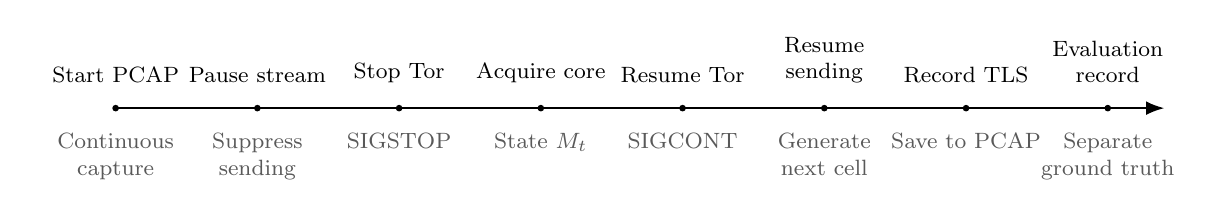
\begin{tikzpicture}[x=18mm,y=1mm,>=Latex,
  event/.style={font=\footnotesize,align=center,text width=20mm},
  arrow/.style={->,thick,TorPurple}]
\draw[arrow] (0,0) -- (7.4,0);
\foreach \x/\top/\bottom in {
  0/{Start PCAP}/{Continuous capture},
  1/{Pause stream}/{Suppress sending},
  2/{Stop Tor}/{\code{SIGSTOP}},
  3/{Acquire core}/{State $M_t$},
  4/{Resume Tor}/{\code{SIGCONT}},
  5/{Resume sending}/{Generate next cell},
  6/{Record TLS}/{Save to PCAP},
  7/{Evaluation record}/{Separate ground truth}}
  {
    \fill[TorPurple] (\x,0) circle (1.2pt);
    \node[event,above=2mm] at (\x,0) {\top};
    \node[event,below=2mm,text=black!65] at (\x,0) {\bottom};
  }
\end{tikzpicture}
\caption{Timeline of experiments that pause communication. Evaluation records are used only for comparison after decryption.}
\label{fig:acquisition-timeline}
\end{figure}

Table~\ref{tab:experiment-groups} summarizes experimental groups and independent units. Because populations and independent units differ by group, results are aggregated separately by group.

\begin{table}[!tbp]
\centering
\caption{Experimental groups, objectives, and independent units}
\label{tab:experiment-groups}
\small
\begin{tabularx}{\linewidth}{Y L{25mm} L{31mm}}
\toprule
Objective and condition & Independent unit & Scale \\
\midrule
Structural recovery across 0.4.9 and optimization variants & Tor process & 12 runs, 144 circuits \\
Lifecycle and remnant structures & Circuit/acquisition point & 12 established, 8 building, 6 terminated \\
End-to-end TLS-record and CGO-layer decryption & Tor process & 10 runs, 7 candidates each \\
Inter-endpoint time gap and preceding cell & Tor process & 3 runs, 36 hops \\
Negative controls: executable, loss, wrong state & Condition & 3 ELFs, 2 losses, 7,168 wrong states \\
Implementation boundary of known resynchronization attack & Tor process & 3 runs \\
Fixed-delay acquisition without pausing stream or observing cell/TLS boundaries & Tor process & 6 runs, 2/3 hops \\
Admission restriction for mixed CGO/\torone{} circuits & Circuit & 19 circuits, 10 mixed \\
Application to official Debian package & Tor process & 3 structural runs/36 circuits; 6 traffic runs \\
\bottomrule
\end{tabularx}
\end{table}

\subsection{Evaluation Items}

The evaluation was divided into six groups.

\begin{enumerate}
  \item Accuracy of owned circuits, entry-oriented paths, and mixed CGO/\torone{} classification.
  \item Reproducibility across version, optimization, LTO, and ABI differences.
  \item Suppression of false acceptance for established, building, and terminated states, missing pages, and mismatched binaries.
  \item Joining streams, circuits, paths, CGO state, and the next cell.
  \item Decryption of TLS records and CGO layers using only a core dump and PCAP as inputs.
  \item Boundaries involving acquisition-time mismatch, preceding cells, wrong keys, and the known backward-direction resynchronization attack.
\end{enumerate}

Circuits and hops are correlated within a process. Repeated-run success rates therefore use a run that reinitializes Tor process state each time as the unit. Two-sided 95\% Wilson score intervals are reported descriptively by treating runs as exchangeable Bernoulli trials. Trials varying hop count or acquisition delay are not random samples from an identical distribution, so these intervals are not used to estimate success rates in general environments. Deterministically generated wrong states receive no confidence interval; only observed counts are reported.

\section{Results}\label{sec:results}

\subsection{Recovery of Circuits and Cryptographic State Satisfying the Validation Conditions}

In the initial real-Tor evaluation, 20/20 circuits in a 0.4.9.16-only environment and 19/19 circuits in an environment mixing 0.4.9.16 and 0.4.8.25 matched Control Protocol circuit IDs. All 39/39 entry-oriented paths also matched.
The 51 hops in the mixed environment were classified as 40 CGO and 11 \torone{}. Every hop containing a 0.4.8.25 relay was \torone{}.
Reanalysis of this mixed core with the proposed method found, among 19 active circuits with validated ownership, path structure, and cryptographic contexts, 8 all-CGO circuits, 10 mixed CGO/\torone{} circuits, and 1 \torone{}-only circuit. The circuits satisfying the conditions for TLS/CGO traffic recovery were exactly the 8 all-CGO circuits. The 10 mixed circuits and 1 \torone{}-only circuit did not satisfy the all-CGO condition.

In the broader evaluation, each of four arm64 conditions was run 3 times, recovering 144/144 controlled circuits and 432/432 hops (Table~\ref{tab:generalization}). All 12 processes succeeded completely, giving a process-level 95\% Wilson interval of 75.75--100\%.

\begin{table}[!tbp]
\centering
\begin{threeparttable}
\caption{Recovery across version and optimization differences}
\label{tab:generalization}
\small
\begin{tabularx}{\linewidth}{Yrrr}
\toprule
Condition & Complete success & Circuits & CGO hops \\
\midrule
0.4.9.3-alpha, \code{-O0} & 3/3 & 36/36 & 108/108 \\
0.4.9.9, \code{-O0}       & 3/3 & 36/36 & 108/108 \\
0.4.9.16, \code{-O0}      & 3/3 & 36/36 & 108/108 \\
0.4.9.16, \code{-O2}      & 3/3 & 36/36 & 108/108 \\
\midrule
Total & 12/12 & 144/144 & 432/432 \\
\bottomrule
\end{tabularx}
\begin{tablenotes}\footnotesize
\item Because circuits and hops are correlated within a process, the process is the unit for independent success rates.
\end{tablenotes}
\end{threeparttable}
\end{table}

\subsection{Application to Official Tor 0.4.9.17}

Table~\ref{tab:packaged} reports application to a distributed package rather than a self-built binary. Tor 0.4.9.17 for Debian 12 arm64 from the Tor Project's official repository was stripped, and the executable's GNU Build ID was \code{59de31af...a9f}. The external debug file in \code{tor-dbgsym} from the same repository matched this Build ID. Across 3 independent runs, the analyzer recovered ownership and entry-oriented paths for 36/36 circuits and established CGO state for 108/108 hops. The two-sided 95\% Wilson score interval for 3/3 process-level successes is 43.85--100\%; this confirms feasibility under a small number of conditions and is not an estimate of success rates across distributed environments generally.

\begin{table}[!tbp]
\centering
\caption{Evaluation of the Tor Project's official Debian package}
\label{tab:packaged}
\small
\begin{tabularx}{\linewidth}{L{29mm}L{18mm}YY}
\toprule
Evaluation & Independent runs & Structure/authentication result & Recovered content \\
\midrule
Structural recovery & 3/3 & 36/36 circuits, 108/108 CGO hops & Ownership and entry order \\
Post-acquisition replay & 6/6 & Unique CGO authentication 6/6 & 5 DATA, 1 SENDME \\
\bottomrule
\end{tabularx}
\end{table}

Without external debug symbols, type information could not be resolved and circuit recovery was not established. When a debug file with a different Build ID was supplied, GDB likewise did not load type information and circuit recovery was not established. In executable-to-core compatibility checking, the correct distributed executable passed with 95.57\% agreement over 368,640 comparable bytes. A different Tor 0.4.9.16 build agreed on only 39.62\% and failed the compatibility condition. Thus, the method cannot be applied from the distributed executable alone, but preserving matching external debug symbols enables ownership-list, circuit-structure, and cryptographic-context validation under the same conditions as a self-built binary.

Traffic recovery was evaluated in 6 further runs using the same distributed executable and debug symbols, rebuilding the isolated network and Tor processes each time. Communication was not paused, and core-dump acquisition began after fixed delays of 0.13, 0.31, 0.57, 0.19, 0.43, and 0.71 seconds from stream start. Cell processing and TLS-record boundaries were not observed. Three 2-hop and three 3-hop runs each authenticated 1 record corresponding to in-core TLS write-record sequence numbers 13, 16, 19, 25, 29, and 34. Exactly 1 candidate passed CGO authentication in all 6/6 runs. Hop 1 was recognized for 2-hop circuits and hop 2 for 3-hop circuits. Every check from ownership validation through TLS AEAD and unique CGO authentication succeeded in 6/6 runs. Under an exchangeable-Bernoulli assumption, the descriptive 95\% Wilson score interval is 60.97--100\%.

Among the 493-byte CGO-authenticated bodies, 5/6 were relay DATA cells containing the evaluation marker: 2/3 for 2-hop and 3/3 for 3-hop circuits. The remaining 1 run recovered a SENDME relay command that passed CGO authentication but contained no evaluation marker. The descriptive 95\% Wilson score interval for marker-bearing bodies in 5/6 runs is 43.65--96.99\%. Successful CGO authentication does not guarantee recovery of the traffic content sought by an investigator.

The replay tool was built from the Tor Project's official 0.4.9.17 source archive (SHA-256 \code{ff372c41...abe2}). Production source files were unchanged; only the test harness in \code{test_crypto_cgo.c} was extended with an interface for loading stored state. The replay tool's SHA-256 is \code{e71129d0...0acbd} and GNU Build ID is \code{cfebbca1...eebc}. Reprocessing all 36 candidates from the 6 stored runs produced 36/36 agreement with the previous 0.4.9.16-based replay in CGO-authenticated hop, recovered bytes, and the flag indicating no use of ground-truth information.

TLS negative controls authenticated 0 records when 1 bit of the traffic secret was changed or TLS state from a different run was supplied. Incrementing the write sequence number by 1 with the same connection secret authenticated the correct subsequent record. AEAD authentication alone therefore does not identify the record immediately after acquisition; agreement with the in-core number and acquisition order is required.

For automatically generated circuits without explicit paths, 3 runs of 0.4.9.3-alpha contained 133 CGO and 91 \torone{} hops; 0.4.9.9 contained 132 CGO and 93 \torone{} hops. After the fix, 0.4.9.16 contained 438 CGO and 12 \torone{} hops. This distribution difference is consistent with the condition corrected in 0.4.9.12, which had failed to negotiate CGO on non-final hops~\cite{torrelease04912}. Because hop selection and path length were not fixed for automatically generated circuits, these values are not interpreted as network-wide adoption rates. The 432/432 result in Table~\ref{tab:generalization} is a conditional evaluation of whether each version's analyzer can recover known circuits whose CGO contexts were confirmed initialized.

For the LTO build, GDB could not directly obtain the ownership-list location from DWARF. The fallback using an ELF local symbol and PIE load bias recovered 12/12 circuits and 36/36 CGO hops.
The x86\_64 guest core under QEMU also matched 12/12 circuits and 36/36 hops.


The analyzer classified 12/12 established circuits, 8/8 building circuits, and 6/6 circuits absent from the ownership list after normal termination.
The 16 building hops appeared to be \torone{} from enum values alone, but their cryptographic state was uninitialized. Their scheme was therefore indeterminate and did not satisfy the conditions for established \torone{}.

Across 8 conditions that zeroed 4-KiB pages in a complete ELF core, there were 0 false structurally valid candidates. This was simulated loss by zeroing, not genuine missing pages. When the ownership-list \code{smartlist} was zeroed, an analyzer that did not check read success and enumeration completion would interpret the result as 0 circuits without error. Under this condition, however, not every ownership-list element can be confirmed, so circuit absence cannot be determined. With completion checks, the result was ownership list unavailable.

We further evaluated 2 conditions that removed, from the core's program headers, the heap \code{PT_LOAD} containing the ownership-list \code{smartlist} and the executable data \code{PT_LOAD} containing the ownership-list variable, respectively, making them genuinely unreadable. In both conditions, the ownership list was unavailable and circuit structure could not be validated.

Executable matching used 3 conditions: the matching ELF, an LTO build of the same version, and a different version. The matching ELF passed with 84.51\% agreement of mapped bytes; the same-version LTO and different version, at 8.71\% and 9.58\%, failed the compatibility condition. Type resolution did not proceed in the latter 2 conditions, and circuit counts were indeterminate.

For complete core dumps of approximately 731~MiB, median analysis times for 0/12/48/95 controlled circuits were 0.142/0.164/0.223/0.306 seconds. Maximum RSS was 57,404--60,224~KiB. Acquisition paused the process for 1.33--1.47 seconds, and hashing took 0.92--1.04 seconds.

\subsection{Recovery of Traffic after Core-Dump Acquisition}

From client core dumps, the analyzer joined destinations, Control circuit IDs, and entry-oriented paths for 12/12 controlled streams, with 0 false positives and 0 false negatives.
The next relay cell generated after core-dump acquisition was supplied to current CGO state extracted from the same owned circuit. All 5 independent runs recognized hop 2, and 493/493 bytes of the body matched evaluation plaintext.

Negative controls were extended across complete CGO state. For each of 7 categories---the $J$-side AES key, $J$-side POLYVAL key, $S$-side AES key, $S$-side POLYVAL key, nonce, $T'$, and hop order---1,024 states were applied to the same real cell, for 7,168 states in total, with 0 false recognitions. These deterministic controls are not random samples from all wrong states and are therefore not generalized to a confidence interval for the false-positive rate.
For arbitrary-time acquisition during continuous communication, 10 snapshots were collected from each of 3 processes, and CGO-state extraction succeeded in 30/30. Snapshots within a process are correlated. When the 10 snapshots per process are grouped and aggregated at process level, success is 3/3 processes with a 95\% interval of 43.85--100\%.


Decryption inputs were limited to a client core dump corresponding to the acquisition point, a validated executable and type information, and an entry-link PCAP. Ground-truth circuit IDs from the Control Protocol and ground-truth cells from dynamic hooks were excluded from decryption inputs and used only for comparison after candidate selection.

Ten independently acquired datasets were reanalyzed with ownership, path-structure, and cryptographic-context validation as prerequisites for traffic recovery. In 10/10 runs, the ownership list was completely enumerated and all three checks succeeded. Subsequent TLS and CGO validation was performed for all-CGO circuits satisfying these conditions.

Negative controls for bypass included a condition with no circuit having validated cryptographic contexts, conditions missing circuit information required for traffic recovery, and a condition with a modified circuit address. Validation failed under all 4 conditions and 0 secret values were recovered.

For each acquisition, the cipher suite \code{TLS_AES_256_GCM_SHA384} was obtained directly from OpenSSL state, and 1 TLS~1.3 record corresponding to in-core write sequence number 7 was authenticated and decrypted. 7 cells with the target entry-link circuit ID were enumerated without a selector derived from the Control Protocol.

Applying a copy of the same acquisition-time CGO state to every candidate produced exactly 1 candidate per trial whose CGO authentication tag validated, with hop 2 as its destination. After candidate selection, comparison with ground truth confirmed that the authenticated candidate was the correct candidate, that the 509 PCAP-derived bytes matched the dynamically obtained ground truth, and that the 493 bytes excluding the authentication tag matched ground-truth plaintext. Every check in Table~\ref{tab:full}, from complete ownership-list enumeration through post hoc comparison with ground-truth plaintext, succeeded in 10/10 runs.

\begin{table}[!tbp]
\centering
\caption{Validation results from sequential TLS-record and CGO-layer processing}
\label{tab:full}
\small
\begin{tabularx}{\linewidth}{YcL{31mm}}
\toprule
Validation item & Result & Success condition \\
\midrule
Complete ownership-list enumeration & 10/10 & Every element readable \\
Circuit structure and entry-oriented path & 10/10 & Magic, index, bidirectional links, and cycle consistent \\
CGO cryptographic contexts & 10/10 & Initialization and structure consistent at all active hops \\
TLS AEAD and cell extraction & 10/10 & 1 record at sequence 7 and 7 cells each \\
Unique CGO authentication & 10/10 & One authenticated candidate each; CGO hop 2 \\
Post hoc agreement with evaluation ground truth & 10/10 & Candidate, hop, and 493/493 body bytes agree \\
\bottomrule
\end{tabularx}
\end{table}

With the Tor process as the independent unit, the two-sided 95\% Wilson interval for 10/10 repeated successes under fixed conditions is 72.25--100\%.
In additional fixed-delay experiments that neither stopped the stream nor observed cell or TLS boundaries, every check from ownership validation through unique CGO authentication also succeeded in 6/6 runs. CGO authentication succeeded at hop 1 in three runs with 2-hop circuits and at hop 2 in three runs with 3-hop circuits. TLS write-record sequence numbers obtained from the core dumps were 17, 23, 29, 37, 53, and 68, differing in every trial, and one TLS~1.3 record was authenticated at each number. Exactly 1 of 7 cell candidates in each trial passed CGO authentication, after which the evaluation marker also matched. The descriptive 95\% Wilson score interval for 6/6 is 60.97--100\%.

These additional experiments excluded Control Protocol circuit IDs, dynamically hooked cells, ground-truth hops, and ground-truth plaintext from decryption inputs. They therefore reject the possibility that 10/10 success depended only on fixed record number 7, fixed hop 2, or stream pausing. However, Tor did not use a 1-hop general SOCKS stream as an ordinary exit circuit, so traffic decryption with hop 0 as destination could not be evaluated. 0 relay-cell bodies were recovered under wrong-key, different-run secret, cryptographic-context validation failure, modified validated-circuit information, and mixed-circuit conditions. Because all 6 trials succeeded, no failure case for fixed-delay acquisition was observed.

A PCAP-only control without TLS secrets recovered no known cell, plaintext, or synthetic identifier even after reassembling 118 packets and 78 TCP-payload segments.

In TLS negative controls, a 1-bit flip in the client traffic secret and a TLS secret from another run each authenticated 0 records. In contrast, changing the write-record sequence number from 7 to 8 while retaining the same connection secret correctly authenticated the subsequent record numbered 8. AEAD authentication establishes a record's cryptographic validity but not that it is the record immediately after acquisition. Adoption of a TLS record therefore requires an unmodified in-core record sequence number and the acquisition order in Figure~\ref{fig:acquisition-timeline}.

This result is not a claim of decryption from memory alone or from a PCAP alone. It results from joining both pieces of time-corresponding evidence through circuit ownership.

\subsection{Time Gaps Destroyed Cryptographic-State Correspondence before Structural Correspondence}

While a 100-MB stream was transferred over 12 circuits, the client and 3 relays were acquired sequentially.
Even with measured acquisition gaps of 2.297, 2.663, and 3.168 seconds, link sequences corresponded for 36/36 hops. Complete nonce and $T'$ matches, however, were 0/36.
Circuit structure persists for seconds, whereas cryptographic state advances with every cell.

In 3 trials applying current state immediately after cell processing to the preceding forward cell, the CGO-authenticated hop was $-1$ in every case and plaintext did not match. This confirms the temporal boundary in Figure~\ref{fig:time} on real Tor.

\begin{table}[!tbp]
\centering
\caption{Recovery that succeeded and recovery that did not}
\label{tab:boundary}
\small
\begin{tabularx}{\linewidth}{YcY}
\toprule
Question & Result & Interpretation \\
\midrule
Owned circuits and entry-oriented paths & 144/144 & Structural correspondence reproduced \\
Next cell after core-dump acquisition & 5/5 & Current CGO state usable \\
Core dump plus PCAP & 10/10 & Recovery from one TLS record to one relay body per run \\
Unpaused stream, fixed-delay acquisition & 6/6 & Unique CGO authentication across 6 TLS numbers and destination hops 1 and 2 \\
Official package, unique CGO authentication & 6/6 & 5/6 marker-bearing DATA bodies; 1/6 non-marker body \\
Mixed circuits admitted to traffic recovery & 0/10 & All-CGO condition not satisfied \\
Current state plus preceding cell & 0/3 & Past state not generally invertible \\
Sequentially acquired endpoint states & 0/36 & Simultaneous stop required for instantaneous matching \\
Wrong-CGO-state destination misrecognition & 0/7168 & Deterministic controls in 7 categories \\
\bottomrule
\end{tabularx}
\end{table}

\section{Attack-Capability Boundary of Extracted State}\label{sec:security}

Extracting cryptographic state from memory does not by itself enable remote attacks or deanonymization. To examine this threat boundary, we reproduced Pillwax's IPR-plus-resynchronization distinguishing attack against backward CGO in C Tor 0.4.9.16 and tested how far it progressed on a real 3-hop circuit~\cite{pillwax2026improving}. This is not a separate vulnerability claim from the proposed method; it is a boundary experiment measuring capabilities that must not be extrapolated from extracted state.

For a single middle layer, flipping 1 bit on the right side of a modified cell while retaining its left-side tag caused that cell not to be recognized, but the target layers on the client and relay resynchronized. The next normal cell matched in 509/509 bytes.
Thus, the formal resynchronization property exists in the implementation.

Under 3-hop processing, however, only the outer target layer resynchronized; $T'$ in the 2 inner layers that processed the modified cell no longer matched the relay side. Even if the circuit was artificially preserved, the next normal exit cell was not recognized. Arti 0.48.0 likewise rejected the same 2-cell sequence with \code{BadCellAuth}~\cite{artisource048}.
Furthermore, in 3 independent runs on the isolated Chutney network where the entry relay modified 1 cell once, the client closed the target circuit in 3/3 runs. The 95\% Wilson interval is 43.85--100\%, reflecting the small sample.

The known formal attack is therefore reproducible in the implementation, but in this evaluation it did not develop into keyless decryption, cell forgery, or deanonymization. Mismatch of inner state after full-layer processing and circuit closure at the first authentication failure prevented a second query. This study does not claim a new vulnerability from this result.

\section{Discussion}\label{sec:discussion}

\subsection{Practical Significance and Capability Boundary}

The questions this method directly answers are specific.
It can recover client-originated circuits owned by Tor at acquisition time, their Control circuit IDs, relay order from the entry, per-hop CGO/\torone{} schemes, and initialization and update status of per-direction CGO state.
If stream structures remain, SOCKS destinations can be linked to their owning circuits and paths.
With an entry-link PCAP spanning core-dump acquisition, Tor cells can be extracted from TLS records and processed through CGO to recover relay bodies. The recovery unit is a 493-byte Tor relay-message body. Even if a DATA message contains application bytes, ciphertext from HTTPS or an Onion Service upper-layer protocol requires separate decryption.

This information is suitable for verifying which destination a compromised endpoint connected to at investigation time, which circuit it used, which cryptographic schemes were confirmed initialized, and which relay message it sent immediately after acquisition.
The practical benefit is reproducible analysis of acquired evidence even when ordinary logs lack destinations or content and the Control Port can no longer be queried.

If a plaintext PCAP from the localhost side has already been acquired and the sole objective is application content, that method should be used first, as Table~\ref{tab:practical-alternatives} indicates. The additional value here is not finding plaintext-like fragments, but attributing owned circuits, entry order, hop schemes, TLS records, and CGO-authenticated relay messages from post-termination evidence to the same point in time. Operational deployment requires an acquisition plan covering (1) continuous entry-link PCAP capture, (2) preservation of the Tor binary, shared libraries, and external debug symbols, (3) acquisition of a consistent core dump involving a brief process stop, and (4) access control for secret files.

In evaluation using synthetic source \code{127.0.0.2} and synthetic identifiers, every check agreed for source, stream, destination, circuit ID, 3-hop path, and identifier in decrypted content.
This demonstrates how anonymity metadata is lost when endpoint memory is compromised. It does not identify a real person, externally attribute a source IP, or observe third-party communication.


Decryption of TLS records and CGO layers does not result from cryptanalytic inference of CGO keys. It results from legitimate TLS secrets and CGO state being present in endpoint memory and correctly attributed to a circuit through Tor's ownership relationships.
The threat model therefore includes endpoint-memory read access. The method does not apply to a passive observer holding only a PCAP.

The result does not imply comprehensive decryption of Tor or of past traffic. It demonstrates target- and time-bounded decryption using endpoint state at acquisition.


To compare cryptographic state at both endpoints, target processes should first be stopped simultaneously and memory then saved. Sequential acquisition produces state drift within seconds.
Processing post-dump cells from a client-only core dump and a contemporaneous PCAP does not require simultaneous acquisition of both endpoints. It requires agreement between TLS/CGO state in the core dump and cell order in the PCAP.

To reproduce the experiment's success conditions in field acquisition, investigators must stop Tor while packet capture continues and preserve the core dump, executable, external debug symbols, Build ID, timestamps, and hashes. Analysis must check read success and enumeration completion. If enumeration is incomplete, circuit absence cannot be determined.

\section{Limitations}\label{sec:limitations}

First, evaluation of end-to-end processing from TLS records through CGO layers is limited to Debian arm64, self-built Tor 0.4.9.16 and the Tor Project's official Tor 0.4.9.17 package, OpenSSL 3.0.22, and \code{TLS_AES_256_GCM_SHA384}. Structural recovery on x86\_64 was verified with QEMU guest cores, but end-to-end TLS-to-CGO evaluation on native x86\_64 has not been performed. A change in OpenSSL minor version or provider requires revalidation of the internal profile.

Second, 10/10 success demonstrates repeatability under fixed conditions, and 6/6 self-built fixed-delay trials acquired without observing cell or TLS boundaries extend generalization across TLS record sequence numbers and destination hops. They do not precisely estimate success rates in general environments. Under an exchangeable-Bernoulli assumption, the descriptive 95\% Wilson score intervals are wide: 72.25--100\% and 60.97--100\%, respectively. For the official package, unique CGO authentication succeeded in 6/6 with an interval of 60.97--100\%. Relay DATA-cell bodies containing the evaluation marker were recovered in 5/6, with an interval of 43.65--96.99\%. Additional trials include destination hops 1 and 2, but destination hop 0 and different cipher suites remain unevaluated. The schemes of 10 mixed circuits were classified, but layer-by-layer traffic recovery was not evaluated.

In the 10 communication-paused trials, Tor received \code{SIGSTOP} before core-dump acquisition. The additional 6 trials did not stop the stream or align the stop time with cell or TLS-record boundaries, but \code{gcore} still stopped the process while copying memory. We did not evaluate live memory acquisition without stopping execution or acquisition tools that collect inconsistent pages during instruction execution. The results therefore show that recovery is possible from a consistent snapshot acquired during controlled, ongoing communication by unmodified C Tor, but do not guarantee non-atomic memory acquisition generally.

Third, the evaluation does not cover KeyUpdate, incomplete PCAPs, partial TCP overlap, IP fragmentation, IPv6, pcapng, backward traffic, or long replay of multiple consecutive cells. The implementation's TCP reassembly deduplicates only complete retransmissions with identical sequence numbers. Although current state did not decrypt the preceding cell, the general possibility of another copy of old state or remnants in memory-allocator regions cannot be excluded.

Fourth, package evaluation is limited to one official Tor Project Debian 12 arm64 package and external debug symbols from the same repository. The ownership list, path structure, and cryptographic contexts were validated in 3/3 runs. In another 6/6 runs, TLS AEAD and unique CGO authentication succeeded, but relay DATA-cell bodies containing the evaluation marker were recovered in 5/6. Other distributions, field evidence for which external debug symbols cannot be obtained, and different TLS cipher suites were not evaluated. We therefore do not claim direct applicability to arbitrary distributed Tor binaries.

Fifth, the method uses C Tor types and ownership relationships and does not directly apply to Arti's Rust types. Although sequential CGO state in C Tor and Arti was confirmed to agree for normal operation sequences, Arti requires a separate analyzer for Rust ownership relationships.

Sixth, the literature survey is a scoping review of principal specifications, peer-reviewed papers, implementations, and theses. A systematic review including unpublished tools and non-English literature has not been completed. We therefore make no ``first in the world'' claim.

Finally, this study used only a controlled isolated network and synthetic identifiers. It did not demonstrate identification of individuals, wide-area passive surveillance, or remote deanonymization. These capabilities must not be extrapolated from the results.

\section{Conclusion}

This study presented a memory-forensic method that follows Tor's own ownership relationships to circuits, entries, hops, TLS, and CGO rather than searching for Tor cryptographic state as ``key-like bytes.''
It recovered 144/144 circuits and 432/432 hops across multiple self-built C Tor 0.4.9-series configurations. It also recovered 36/36 circuits and 108/108 hops from the Tor Project's official Debian package.

Traffic recovery from a client core dump and PCAP corresponding to the same acquisition point was reproduced in 10/10 independent self-built runs that paused the stream and in 6/6 independent self-built runs acquired after a fixed delay without observing cell or TLS boundaries. In 6 official-package runs, a unique CGO-authenticated relay-cell body was recovered in 6/6. 5/6 were relay DATA-cell bodies containing the evaluation marker. Because the remaining 1 run produced a different CGO-authenticated relay-cell body, we do not claim that the desired traffic content is always obtained.

Traffic recovery requires validated ownership, path structure, and cryptographic contexts, with CGO established at every hop. Evaluation ground truth was separated from decryption, and ground-truth circuit IDs from the Control Protocol were not used for candidate selection. 10 mixed CGO/\torone{} circuits did not satisfy the all-CGO condition, and their traffic recovery remains unevaluated.
The method thereby verifies the correspondence among a stored PCAP, TLS records, Tor circuits, CGO hops, and 493-byte relay bodies.

The scope of validity is equally clear. Current CGO state is not a key that comprehensively unlocks past traffic. The immediately preceding cell could not be decrypted in 3/3 trials, and sequential acquisition during activity produced 0/36 state matches. The known backward resynchronization attack likewise did not lead to keyless decryption or deanonymization because of 3-hop processing and circuit closure.

Further generalization requires evaluation of native x86\_64, different OpenSSL providers, TLS KeyUpdate, incomplete PCAPs, backward traffic, and Arti ownership structures. Any extension must state not only the range of decryption but also the evidentiary conditions, point in time, and circuit that can be explained.

\printbibliography[title={References}]

\end{document}
